\documentclass[11pt,a4paper]{article}

% ------------------------------------------------------------------ packages
\usepackage[T1]{fontenc}
\usepackage[utf8]{inputenc}
\usepackage{lmodern}
\usepackage{microtype}
\usepackage[margin=2.3cm]{geometry}
\usepackage{amsmath,amssymb}
\usepackage{graphicx}
\usepackage{booktabs}
\usepackage{tabularx}
\usepackage{float}
\usepackage{caption}
\usepackage{subcaption}
\usepackage[table]{xcolor}
\usepackage{fancyhdr}
\usepackage{hyperref}

\graphicspath{{figures/}}
\hypersetup{colorlinks=true, linkcolor=blue!50!black, urlcolor=blue!50!black, citecolor=blue!50!black}
\captionsetup{font=small, labelfont=bf}
\newcolumntype{Y}{>{\raggedright\arraybackslash}X}
\renewcommand{\arraystretch}{1.15}
\setlength{\parskip}{0.45em}
\setlength{\parindent}{0pt}

% a simple float for the algorithms (no extra packages needed)
\newfloat{algo}{tbp}{loa}
\floatname{algo}{Algorithm}
\newcommand{\kw}[1]{\textbf{#1}}

\pagestyle{fancy}
\fancyhf{}
\lhead{\small Multiagent Planning}
\rhead{\small\thepage}
\renewcommand{\headrulewidth}{0.4pt}

% ================================================================== title
\title{\textbf{Multiagent Planning}\\[0.6em]
\large Assignment 1 --- Autonomous Systems}
% TODO: replace with your own details
\author{Diwanshu Yadav, Devesh Bhardwaj, Deepanshu, Sachin Kumar \\ Roll No.\ B23CS1017, B23CS1014, B23CS1012, B23CM1033 \\ \texttt{}}
\date{\today}

\begin{document}
\maketitle
\thispagestyle{empty}

% ================================================================== abstract

\tableofcontents
\newpage

% ================================================================== 1
\section{Introduction}

Automated warehouses use fleets of mobile robots that share a grid of aisles. The fleet's routes are
planned jointly with a \emph{multi-agent pathfinding} (MAPF) algorithm so that no two robots collide.
In practice the environment does not stay as planned: an aisle cell is blocked by a fallen box, a robot
breaks down, or a robot is given an urgent order. Re-running the MAPF planner for the whole fleet after
every such event is expensive, and it changes the routes of many robots that were not affected at all.

This report describes a system that repairs plans \emph{locally}. Its design goals, taken from the
assignment, are:
\begin{enumerate}
  \item agents plan with a multi-agent pathfinding algorithm (Space-Time A*);
  \item disrupted agents communicate with neighbouring agents to negotiate alternative paths;
  \item the repair never re-invokes the multi-agent planner from scratch;
  \item the repair changes the plans of as few agents as possible.
\end{enumerate}
The system is evaluated on the total time steps needed by all agents, on the number of agents whose
plans change for a single disruption, and on how both scale with the number of agents and the density of
dynamic obstacles. Section~\ref{sec:failures} reports the settings in which the agents fail to complete
their tasks.

\paragraph{Summary of results.}
Table~\ref{tab:summary} maps each requirement of the assignment to the section that answers it.

\begin{table}[H]
\centering\small
\caption{Requirements of the assignment and where they are addressed.}
\label{tab:summary}
\begin{tabularx}{\textwidth}{@{}p{3.6cm}p{1.4cm}Y@{}}
\toprule
Requirement & Section & Result \\
\midrule
Total time steps of all agents & \ref{sec:agents}--\ref{sec:tasks} &
Sum of costs grows linearly with the fleet (676 steps for 5 robots to 7{,}490 for 50). Disruptions add
4--13\% at density 1\% and about 21\% at density 10\%. Local repair costs at most 1.1\% more total time
than a full replan over whole runs. \\
Agents whose plans change for one disruption & \ref{sec:single} &
1.1--3.5 robots with local repair for 10--50 robots, against 2.8--45 for a full replan. \\
Effect of the number of agents & \ref{sec:agents}, \ref{sec:bigmap} &
Changed plans per event grow from 1.1 to 2.1 between 5 and 100 robots; a full replan grows from 2.3 to
28.7. \\
Effect of obstacle density & \ref{sec:density} &
Extra time grows linearly with density; changed plans per event stay at about 1.4. \\
Failure settings & \ref{sec:failures} &
Dense dynamic obstacles with large fleets cause deadlocks; permanent breakdowns and permanently blocked
cells or stations make tasks impossible. \\
Graphical demonstration & \ref{sec:vis} & Nine animations, including two failure cases. \\
\bottomrule
\end{tabularx}
\end{table}

% ================================================================== 2
\section{Problem Formulation}

\paragraph{Environment.} The warehouse is a 4-connected grid $G=(V,E)$ of free cells; shelf cells are
static obstacles. Time is discrete, $t=0,1,2,\dots$

\paragraph{Agents and tasks.} Robot $i$ starts at its home cell $h_i$ and is assigned an ordered list
of tasks $\langle (p_{i1},d_{i1}),\dots,(p_{ik},d_{ik})\rangle$, where $p$ is a pickup cell next to a
shelf and $d$ is a delivery station. Picking up and dropping off each take one time step. When all its
tasks are done, the robot returns to $h_i$ and parks there. At every step a robot moves to a neighbouring
cell or waits.

\paragraph{Plans and conflicts.} A plan is a sequence $\pi_i = (\pi_i(0),\pi_i(1),\dots)$ of cells. Two
plans conflict if
\begin{align*}
\text{vertex conflict:}\quad & \pi_i(t)=\pi_j(t), \\
\text{edge (swap) conflict:}\quad & \pi_i(t)=\pi_j(t{+}1) \;\wedge\; \pi_i(t{+}1)=\pi_j(t).
\end{align*}

\paragraph{Disruptions.} Three kinds of disruption occur during execution (Table~\ref{tab:disruptions}).
To find the limits of the system, two \emph{permanent} variants are also modelled: a robot that breaks
down for good, and a cell that is blocked for good.

\begin{table}[H]
\centering\small
\caption{Disruption models.}
\label{tab:disruptions}
\begin{tabularx}{\textwidth}{@{}p{3.2cm}Y@{}}
\toprule
Disruption & Model \\
\midrule
Cell blockage & A free cell becomes impassable for $d\in[10,20]$ steps. It is announced when it starts. \\
Agent breakdown & A robot stops where it is for $d\in[10,20]$ steps and is an obstacle to all others. \\
Emergency task & A robot receives a high-priority pickup and delivery, inserted at the front of its
queue (or right after its current delivery if it is carrying an object). \\
Permanent breakdown & The robot never recovers; its undelivered tasks are lost. \\
Permanent blockage & The cell never frees up again. \\
\bottomrule
\end{tabularx}
\end{table}

\paragraph{Objectives.}
The \emph{sum of costs} $\mathrm{SoC}=\sum_i T_i$, where $T_i$ is the time step of robot $i$'s last
delivery, is the total time required by all agents. The \emph{plan-change count} of a disruption is the
number of robots whose future plan differs after the repair. The repair must keep every plan
conflict-free, must not re-run the multi-agent planner, and should keep the plan-change count small.

% ================================================================== 3
\section{System Design}

\subsection{Warehouse map}
The default map is an $18\times35$ grid with 438 free cells: 24 shelf blocks of $2\times4$ cells,
one-cell-wide vertical aisles and two-cell-wide horizontal aisles; 248 pickup cells next to shelves;
14 delivery stations on the left and right edges; and 70 home cells on the top and bottom rows. Rows 1
and $H{-}2$ stay free as corridors, so a parked robot never walls anything off. Exp G uses a larger
$26\times55$ map with 60 shelf blocks and 110 home cells.

\subsection{Shared space-time reservation table}
Every committed plan is stored in a reservation table with
vertex reservations $(v,t)$, edge reservations $(u\!\to\!v,t)$ used to detect swaps, and a parking
reservation $(v,\,t\ge t_0)$ for a robot that has finished its route. The table allows several owners
per entry. After a disruption, a robot's old plan may overlap a new constraint (for example, a broken
robot now occupying a cell); that overlap is exactly how the system identifies the robots whose plans
have become invalid.

\subsection{Initial planning: prioritized Space-Time A*}
\begin{itemize}
  \item \textbf{Space-Time A*} searches over states $(v,t)$ with five actions (four moves and wait).
  The heuristic is the exact shortest-path distance on the static map, precomputed by BFS, so it is
  admissible and consistent. Reserved vertices, swap edges and known blockages are obstacles.
  \item A pickup or drop goal counts as reached only if the robot can also stay on it for the service
  step. The home goal counts as reached only if the robot can park there forever.
  \item Once $t$ exceeds the last reserved time step the world is static, so states $(v,t)$ and
  $(v,t')$ are merged. This keeps the search finite even when the goal is unreachable.
  \item \textbf{Multi-leg routes:} the legs $p_1\to d_1\to p_2\to\dots\to h$ are chained; each leg starts
  where and when the previous one ended.
  \item \textbf{Prioritized planning (Cooperative A*):} robots plan one after another, each treating the
  plans of the robots before it as moving obstacles. If a robot fails, it is moved to the front of the
  order and the rest are shuffled.
\end{itemize}

\subsection{Detecting the disrupted robots}
A disruption at time $t$ is detected purely by querying the reservation table (Table~\ref{tab:detect});
the planner is not involved.

\begin{table}[H]
\centering\small
\caption{Directly disrupted robots for each disruption type.}
\label{tab:detect}
\begin{tabularx}{\textwidth}{@{}p{4.6cm}Y@{}}
\toprule
Disruption & Directly disrupted robots \\
\midrule
Blockage of cell $c$ during $[t,t+d)$ & Owners of any reservation on $(c,t')$, $t'\in[t,t+d)$ \\
Breakdown of robot $a$ at cell $p$ & Robot $a$ (forced stay at $p$ until $t+d$) and every robot with a
reservation on $p$ during the stay \\
Emergency for robot $a$ & Only robot $a$ \\
Permanent breakdown / blockage & Every robot whose plan becomes invalid; tasks whose pickup or station is
now unreachable are dropped (checked by BFS on the static map minus permanent obstacles) \\
\bottomrule
\end{tabularx}
\end{table}

\subsection{Local plan repair}
Each disrupted robot is repaired in order of its first clash, using escalating levels
(Table~\ref{tab:levels}). Robots that are down are frozen and are never asked to move.

\begin{table}[H]
\centering\small
\caption{Repair levels.}
\label{tab:levels}
\begin{tabularx}{\textwidth}{@{}p{3.1cm}Yp{3.6cm}@{}}
\toprule
Level & What happens & Plans changed \\
\midrule
L0: wait insertion & Keep the original route and insert waits before the conflict until the rest of the
plan is valid. & Only the disrupted robot \\
L1: solo detour & Space-Time A* from the current $(v,t)$ over the remaining legs, with all other plans as
hard constraints. & Only the disrupted robot \\
L2: negotiation & Ask neighbouring robots to give way (Algorithm~\ref{alg:negotiate}). & The disrupted
robot and the neighbours that accept \\
\bottomrule
\end{tabularx}
\end{table}

The robot takes the better of L0 and L1 and accepts it if its delay is at most $\tau=8$ steps;
otherwise it tries L2. If L2 fails it keeps the L0/L1 result.

\begin{algo}[H]
\centering
\fbox{\begin{minipage}{0.93\textwidth}\small
\kw{procedure} \textsc{RepairAgent}$(a, t)$\\[2pt]
\hspace*{1em}1.\ $c \leftarrow$ best of \textsc{WaitInsert}$(a)$ and \textsc{SoloDetour}$(a)$ \hfill(L0 / L1)\\
\hspace*{1em}2.\ \kw{if} $c$ exists \kw{and} delay$(c)\le\tau$ \kw{then} commit $c$; \kw{return} success\\
\hspace*{1em}3.\ \kw{for} $R \in \{4, 8, 16\}$ \kw{do} \hfill(L2, widening radius)\\
\hspace*{2em}\kw{if} \textsc{Negotiate}$(a, t, R, \text{depth}=2)$ \kw{then return} success\\
\hspace*{1em}4.\ \kw{if} $c$ exists \kw{then} commit $c$; \kw{return} success\\
\hspace*{1em}5.\ \kw{return} \textsc{Negotiate}$(a, t, \infty, \text{depth}=3)$ \hfill(last local resort)\\[6pt]
\kw{procedure} \textsc{Negotiate}$(a, t, R, \text{depth})$\\[2pt]
\hspace*{1em}1.\ $N \leftarrow$ non-broken robots within Manhattan distance $R$ of $a$; send REQUEST to $N$\\
\hspace*{1em}2.\ $\pi \leftarrow$ Space-Time A* for $a$ where reservations of $N$ are \emph{soft}
(cost $\tau$ per conflict)\\
\hspace*{1em}3.\ mark the undo log; commit $\pi$; $B \leftarrow$ robots in $N$ that $\pi$ conflicts with\\
\hspace*{1em}4.\ \kw{for each} $b\in B$ (nearest first) \kw{do} \hfill(PROPOSE)\\
\hspace*{2em}\kw{if} \textsc{Solo}$(b)$ has delay $\le 30$ \kw{then} commit it \hfill(ACCEPT)\\
\hspace*{2em}\kw{else if} depth $>0$ \kw{and} \textsc{Negotiate}$(b,t,R,\text{depth}-1)$ \kw{then} continue\\
\hspace*{2em}\kw{else} roll back to the mark; \kw{return} failure \hfill(REJECT)\\
\hspace*{1em}5.\ \kw{return} success
\end{minipage}}
\caption{Local repair with negotiation. All commits go through an undo log, so a negotiation is
all-or-nothing.}
\label{alg:negotiate}
\end{algo}

\paragraph{Negotiation protocol.}
\begin{enumerate}
  \item \textbf{REQUEST:} the disrupted robot $A$ broadcasts to every non-broken robot within
  communication radius $R$ (Manhattan distance). $R$ starts at 4 and widens to 8 and 16 if needed.
  \item $A$ plans with Space-Time A* where the neighbours' reservations are soft: violating one costs
  $\tau$. The search minimises $\text{time}+\tau\cdot\#\text{conflicts}$, so $A$ disturbs a neighbour
  only if this saves more than $\tau$ steps.
  \item \textbf{PROPOSE:} $A$ commits its path and sends it to each neighbour $B$ it conflicts with.
  \item \textbf{ACCEPT / REJECT:} $B$ accepts if it can repair itself with L0/L1 at a delay of at most 30
  steps; otherwise it may negotiate recursively (depth $\le 2$, robots already in the coalition cannot be
  asked again). If anyone rejects, the whole coalition is rolled back and $A$ retries with a wider radius.
  \item \textbf{Emergency robot:} it accepts a solo detour if it arrives within 2 steps of the static
  lower bound; otherwise it negotiates with priority (conflict penalty 1), so neighbours make way.
\end{enumerate}

\paragraph{When every local option fails.} The simulator has two modes:
\begin{itemize}
  \item \emph{Purely local} (\texttt{fallback=False}): the multi-agent planner is never called. The
  disruption is declared unrepairable, the run halts, and undelivered tasks count as failed.
  Section~\ref{sec:failures} uses this mode.
  \item \emph{Safety net} (\texttt{fallback=True}, used in Exps A--H): the global planner is called once
  for this event. This happened for only 5 of 32{,}120 disruptions (0.016\%); in every other case the
  multi-agent planner was \textbf{not} re-invoked.
\end{itemize}

\paragraph{Invariant.} After every repair all plans are conflict-free with each other and with all known
blockages; in test mode this is asserted after every event. The simulator also checks for vertex
collisions, swap collisions and robots on blocked cells at every step.

\subsection{Baseline: full replan}
For comparison, the baseline re-runs the whole prioritized planner after every disruption, for every robot
that still has work (emergency robot first, then broken robots, then the rest by id). It runs on exactly
the same scenarios.

% ================================================================== 4
\section{Experimental Setup}

Unless stated otherwise each robot has 3 tasks with random pickup cells and stations, and each run
continues until all tasks are delivered and all robots are parked. The \emph{dynamic-obstacle density}
$\rho$ is the expected fraction of free cells blocked at any moment; blockages arrive as a Poisson process
with rate $\rho\cdot N_{\text{free}}/15$ per step and last 10--20 steps. Every disrupted scenario is
compared with the same scenario without disruptions.

\paragraph{Metrics.} Sum of costs (total time of all agents); makespan; \emph{extra time} (sum of costs
minus that of the undisturbed run); \emph{agents changed} (robots whose future plan differs after the
event, measured by comparing every plan before and after); \emph{collateral} (changed robots that the
disruption did not hit directly); messages and CPU time per event.

\begin{table}[H]
\centering\small
\caption{Experiments. All values are reported as means with 95\% confidence intervals.}
\label{tab:experiments}
\begin{tabularx}{\textwidth}{@{}p{3.3cm}p{4.6cm}Yp{0.9cm}@{}}
\toprule
Experiment & Varied & Fixed & Seeds \\
\midrule
A: single disruption & $N\in\{10,\dots,50\}$ $\times$ 3 types & one event at $t\in[10,30]$ hitting a moving robot & 30 \\
B: number of agents & $N\in\{5,10,20,30,40,50\}$ & $\rho=1\%$, 2 breakdowns, 1 emergency & 30 \\
C: obstacle density & $\rho\in\{0,\dots,10\}\%$ & $N=20$, 2 breakdowns, 1 emergency & 30 \\
D: delay tolerance & $\tau\in\{0,2,4,8,16,32,\infty\}$ & $N=40$, one event, local repair & 30 \\
E: comm.\ radius & $R\in\{1,2,4,8,16,\infty\}$ & $N=40$, one event, local repair & 30 \\
F: simultaneous breakdowns & $k\in\{1,2,4,8,12\}$ & $N=30$ & 30 \\
G: bigger map & $N\in\{25,50,75,100\}$ & $26\times55$ map, $\rho=1\%$ & 10 \\
H: tasks per robot & 1, 3, 5, 8 & $N=20$, $\rho=1\%$ & 30 \\
I: failure settings & $\rho\le30\%$ $\times$ $N\le70$; permanent disruptions & see Section~\ref{sec:failures} & 20--30 \\
\bottomrule
\end{tabularx}
\end{table}

Exps A--H comprise 3{,}320 runs (plus an undisturbed reference for each); Exp I adds 2{,}630 runs. There
were \textbf{0 collisions and 0 timeouts} in all 5{,}950 runs, and every task was delivered in Exps A--H.

% ================================================================== 5
\section{Results}

\subsection{Impact of a single disruption (Exp A)}\label{sec:single}

\begin{figure}[H]
\centering
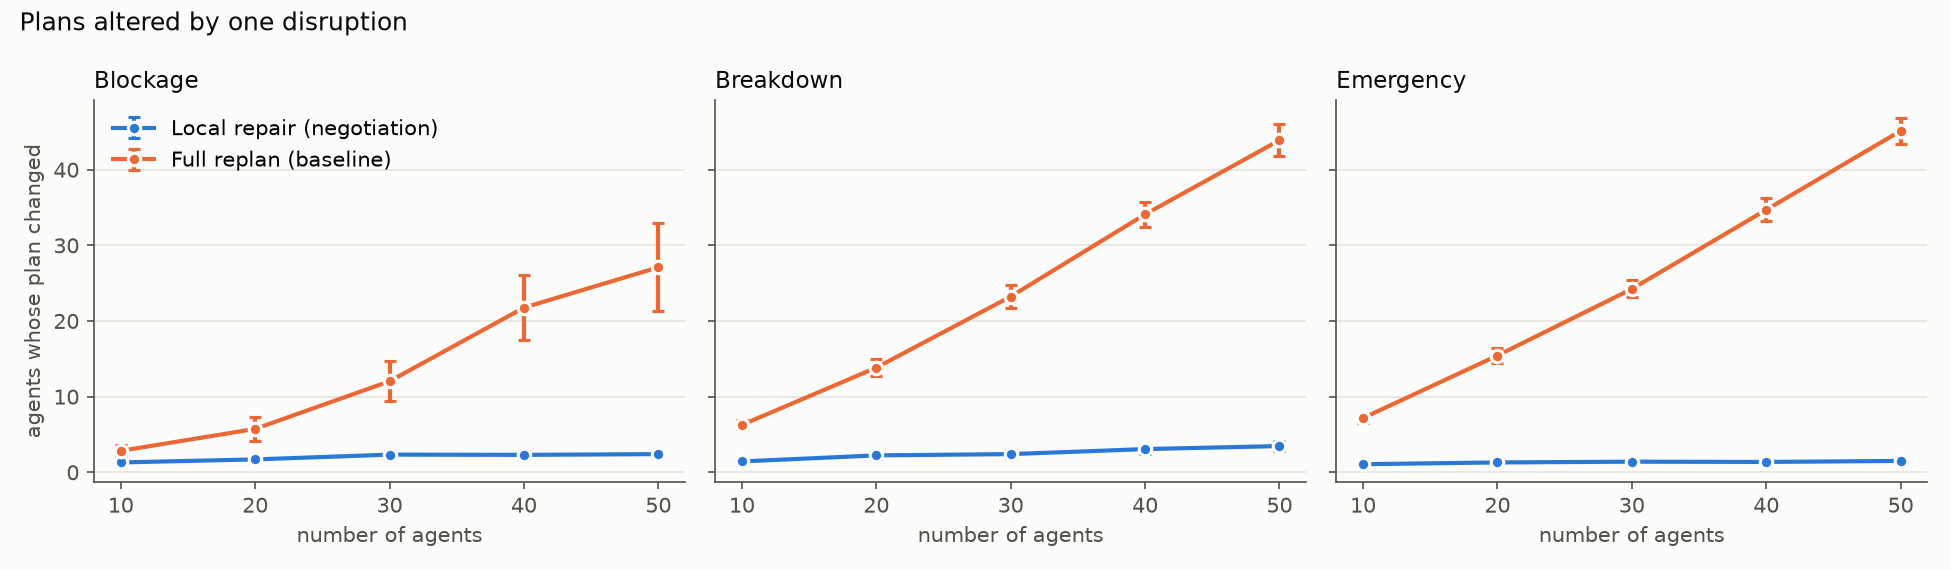
\includegraphics[width=\textwidth]{single_changed.png}
\caption{Number of robots whose plans change to handle one disruption, local repair vs.\ full replan.}
\label{fig:single}
\end{figure}

\begin{table}[H]
\centering\small
\caption{Robots whose plans change for one disruption (mean $\pm$ 95\% CI).}
\label{tab:single}
\begin{tabular}{@{}llccc@{}}
\toprule
Disruption & $N$ & Local repair & of which collateral & Full replan \\
\midrule
Blockage  & 10 & $1.30\pm0.19$ & 0.00 & $2.83\pm0.76$ \\
Blockage  & 30 & $2.33\pm0.47$ & 0.03 & $12.03\pm2.64$ \\
Blockage  & 50 & $2.40\pm0.44$ & 0.13 & $27.10\pm5.80$ \\
Breakdown & 10 & $1.43\pm0.26$ & 0.00 & $6.27\pm0.59$ \\
Breakdown & 30 & $2.40\pm0.54$ & 0.00 & $23.23\pm1.54$ \\
Breakdown & 50 & $3.47\pm0.62$ & 0.17 & $43.90\pm2.13$ \\
Emergency & 10 & $1.07\pm0.09$ & 0.07 & $7.17\pm0.60$ \\
Emergency & 30 & $1.40\pm0.26$ & 0.40 & $24.23\pm1.13$ \\
Emergency & 50 & $1.50\pm0.29$ & 0.50 & $45.13\pm1.73$ \\
\bottomrule
\end{tabular}
\end{table}

With local repair, 1--3.5 robots change their plans per disruption as the fleet grows from 10 to 50, and
most of them are robots the disruption hit directly: on average at most 0.5 extra robots are asked to give
way. A full replan changes 27--45 of 50 plans, because re-running prioritized planning reshuffles everyone.
Across the 450 single-disruption repairs, the levels used were L1 detour 274, L2 negotiation 165, L2
priority (emergency) 118, yield by a neighbour 67, recursive yield 2 and L0 wait 1.

\begin{figure}[H]
\centering
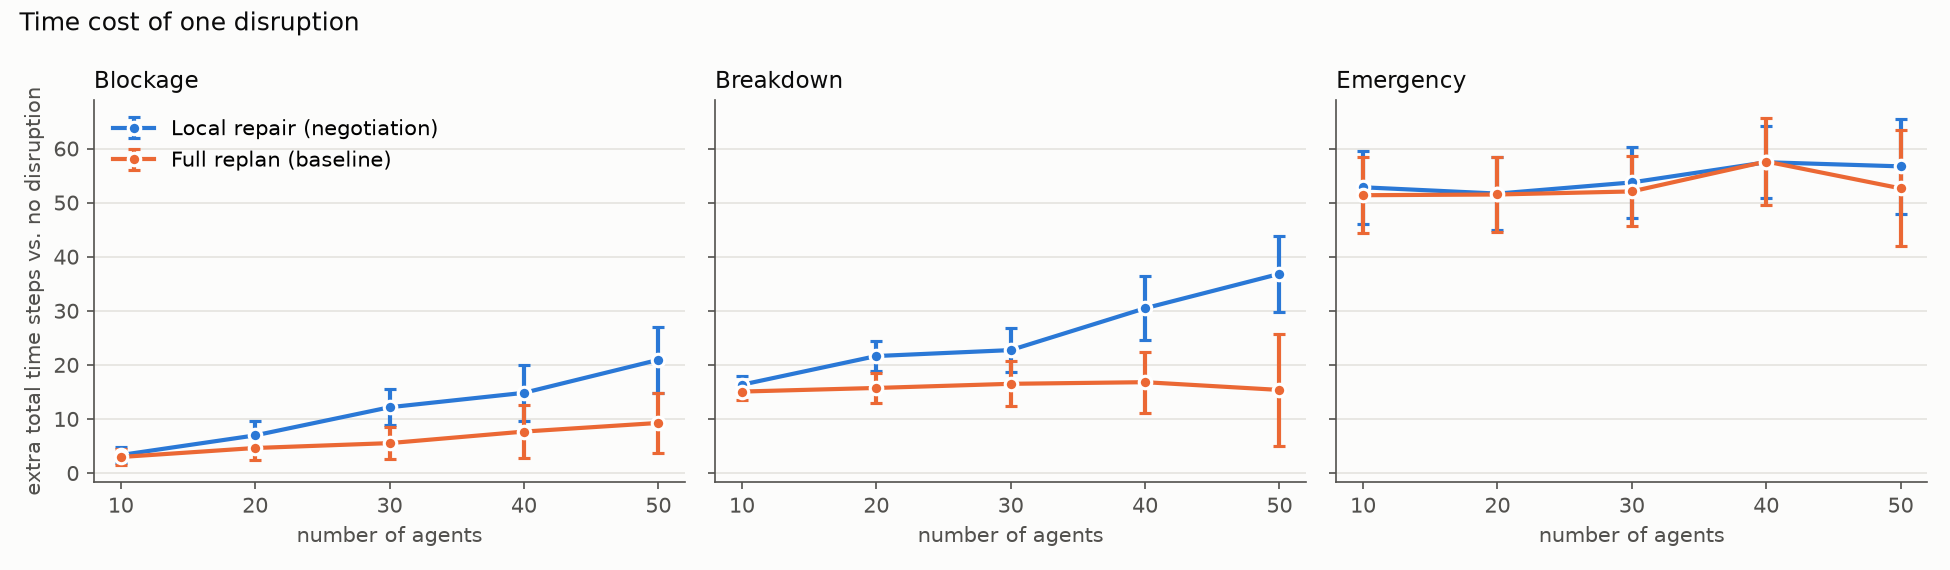
\includegraphics[width=\textwidth]{single_extra_steps.png}
\caption{Extra total time caused by one disruption.}
\label{fig:single-time}
\end{figure}

\textbf{Price of stability.} Keeping the other plans fixed costs some time: with 50 robots one breakdown
adds $36.8\pm7.0$ steps under local repair and $15.4\pm10.4$ under a full replan, which can reorder
priorities globally. For emergencies both cost about the same (51--58 steps), mostly the new task itself.

\subsection{Scaling with the number of agents (Exp B)}\label{sec:agents}

\begin{figure}[H]
\centering
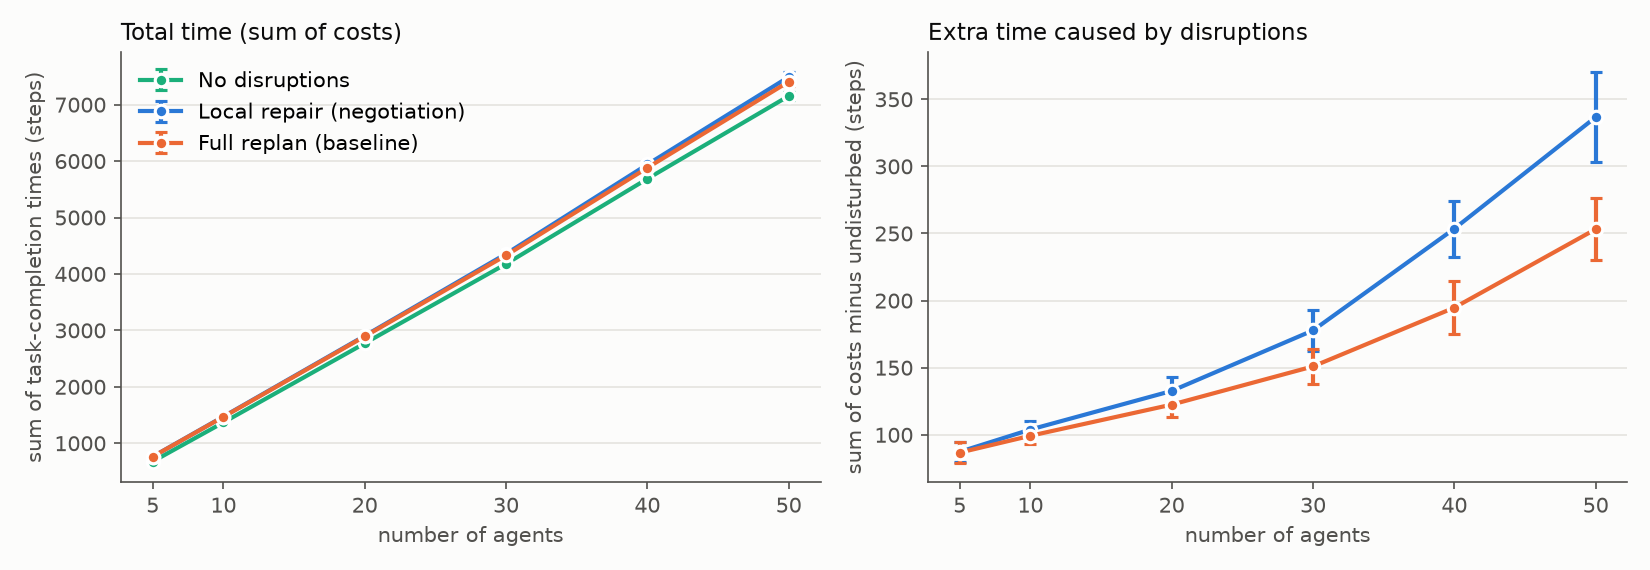
\includegraphics[width=\textwidth]{agents_time.png}
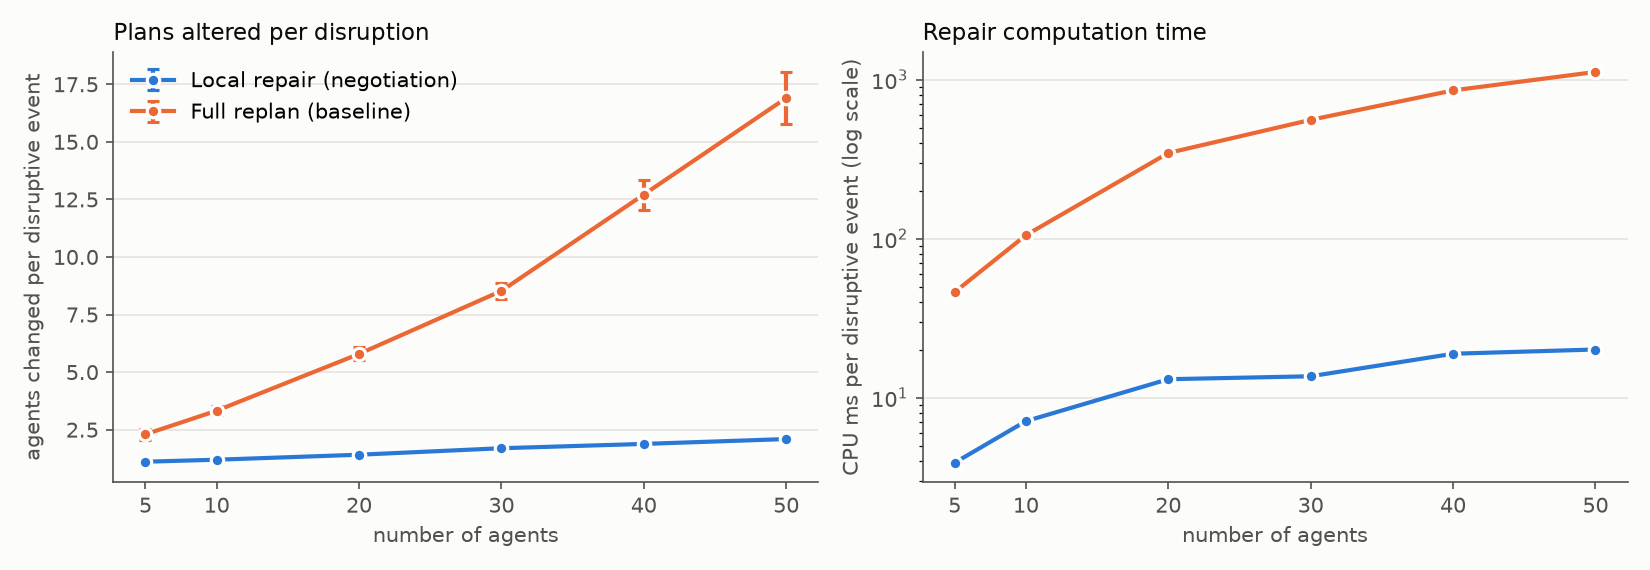
\includegraphics[width=\textwidth]{agents_changes.png}
\caption{Effect of the number of agents ($\rho=1\%$, 2 breakdowns, 1 emergency): total time (top) and
plans changed and CPU time per disruptive event (bottom).}
\label{fig:agents}
\end{figure}

\begin{table}[H]
\centering\small
\caption{Number of agents. SoC = sum of costs (total time steps of all agents).}
\label{tab:agents}
\begin{tabular}{@{}rrrrrrrrr@{}}
\toprule
& \multicolumn{3}{c}{Sum of costs} & \multicolumn{2}{c}{Plans changed / event} & \multicolumn{2}{c}{CPU ms / event} \\
\cmidrule(lr){2-4}\cmidrule(lr){5-6}\cmidrule(lr){7-8}
$N$ & undisturbed & repair & replan & repair & replan & repair & replan \\
\midrule
5  & 676  & 763  & 762  & 1.11 & 2.30  & 3.9  & 46 \\
10 & 1368 & 1472 & 1468 & 1.20 & 3.33  & 7.1  & 105 \\
20 & 2771 & 2904 & 2893 & 1.41 & 5.79  & 13.1 & 346 \\
30 & 4178 & 4356 & 4329 & 1.70 & 8.53  & 13.6 & 559 \\
40 & 5686 & 5940 & 5881 & 1.88 & 12.71 & 18.9 & 856 \\
50 & 7154 & 7490 & 7407 & 2.09 & 16.90 & 20.1 & 1118 \\
\bottomrule
\end{tabular}
\end{table}

Total time grows roughly linearly with $N$ (each robot has 3 tasks) while the makespan stays at about
198--216 steps. Disruptions add 4--13\% to the total time. Local repair costs about 1\% more total time
than a full replan at $N=50$ (7{,}490 vs.\ 7{,}407), but changes $8.1\times$ fewer plans and is
$56\times$ cheaper to compute.

\subsection{Scaling with dynamic-obstacle density (Exp C)}\label{sec:density}

\begin{figure}[H]
\centering
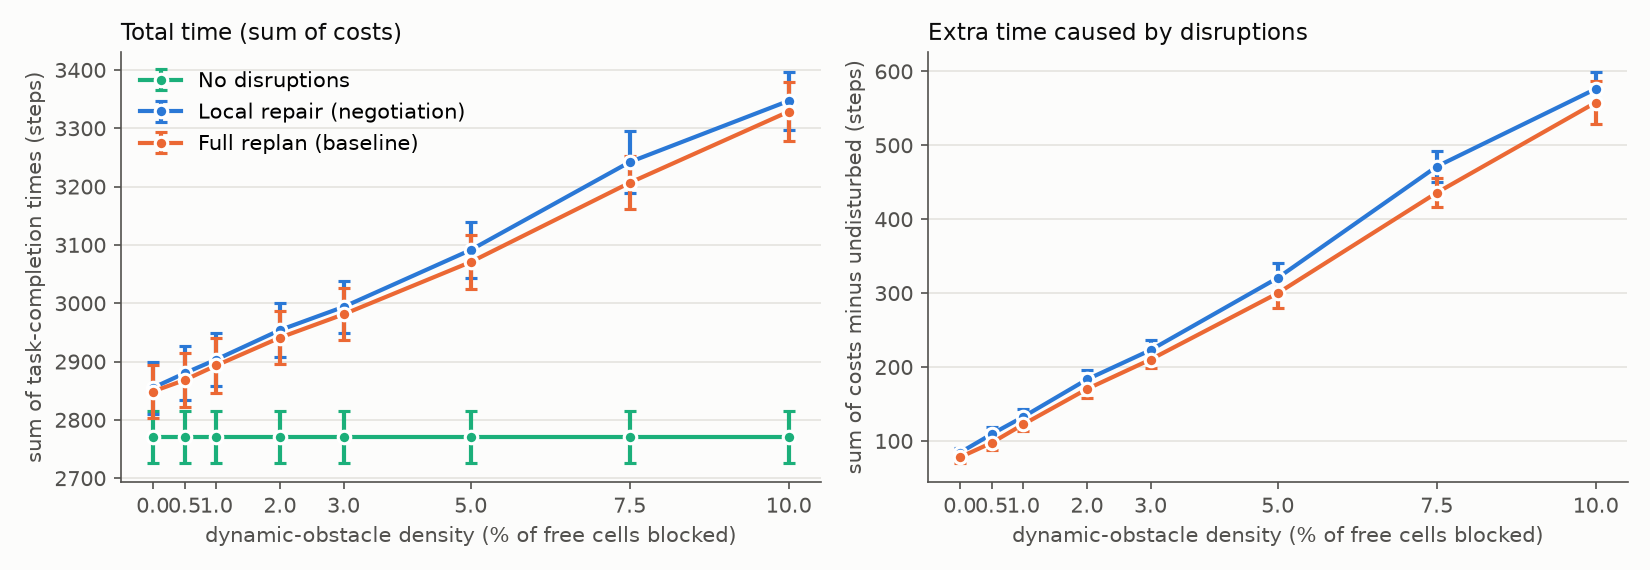
\includegraphics[width=\textwidth]{density_time.png}
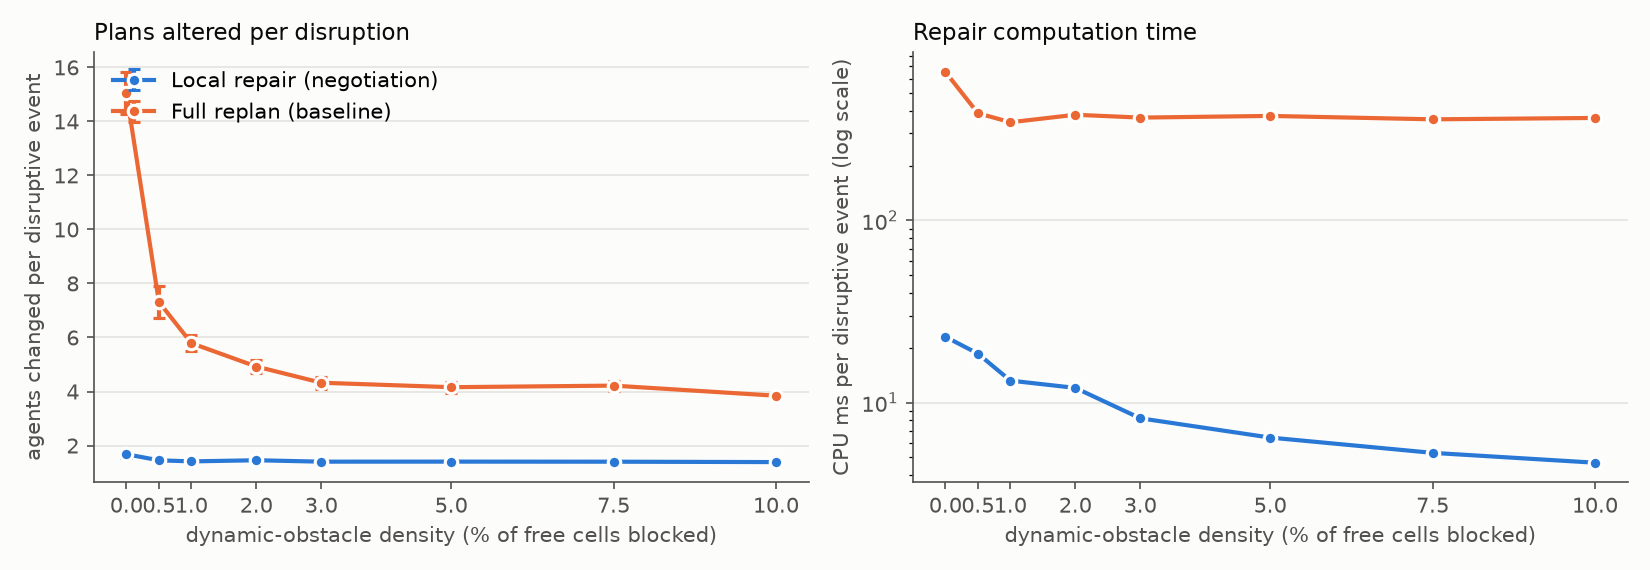
\includegraphics[width=\textwidth]{density_changes.png}
\caption{Effect of the dynamic-obstacle density ($N=20$): total time (top), plans changed and CPU time
per disruptive event (bottom).}
\label{fig:density}
\end{figure}

\begin{table}[H]
\centering\small
\caption{Dynamic-obstacle density ($N=20$).}
\label{tab:density}
\begin{tabular}{@{}rrrrrrrr@{}}
\toprule
& & \multicolumn{2}{c}{Extra time} & \multicolumn{2}{c}{Plans changed / event} & \multicolumn{2}{c}{CPU ms / event} \\
\cmidrule(lr){3-4}\cmidrule(lr){5-6}\cmidrule(lr){7-8}
$\rho$ & disruptive events & repair & replan & repair & replan & repair & replan \\
\midrule
0\%   & 3.0   & 84  & 78  & 1.68 & 15.06 & 23.0 & 653 \\
0.5\% & 13.6  & 109 & 97  & 1.45 & 7.32  & 18.6 & 388 \\
1\%   & 23.4  & 133 & 122 & 1.41 & 5.79  & 13.2 & 346 \\
2\%   & 45.3  & 183 & 170 & 1.46 & 4.92  & 12.0 & 380 \\
3\%   & 66.3  & 223 & 210 & 1.40 & 4.33  & 8.2  & 367 \\
5\%   & 102.0 & 321 & 300 & 1.40 & 4.16  & 6.4  & 375 \\
7.5\% & 162.0 & 471 & 436 & 1.40 & 4.22  & 5.3  & 359 \\
10\%  & 217.8 & 576 & 558 & 1.39 & 3.84  & 4.7  & 365 \\
\bottomrule
\end{tabular}
\end{table}

The number of disruptive events and the extra time grow linearly with $\rho$; at $\rho=10\%$ the extra
time is about 21\% of the undisturbed total for both methods. Local repair changes about 1.4 plans per
event at every density and stays within 1.1\% of the full replan's total time.

\subsection{Delay tolerance and communication radius (Exps D, E)}

A smaller delay tolerance $\tau$ means more negotiation and slightly more changed plans, for at most about
one step less total time (e.g.\ breakdown: 3.43 plans at $\tau=0$ vs.\ 3.07 at $\tau=8$). A wider radius
lets the disrupted robot push aside more neighbours without saving time (Figure~\ref{fig:radius}): for an
emergency, an unlimited radius changes $3.5\times$ more plans and sends $24\times$ more messages than
$R=1$. Negotiating only with close neighbours therefore best meets the goal of minimising changed plans;
the default $R=4$ costs almost nothing over $R=1$.

\begin{figure}[H]
\centering
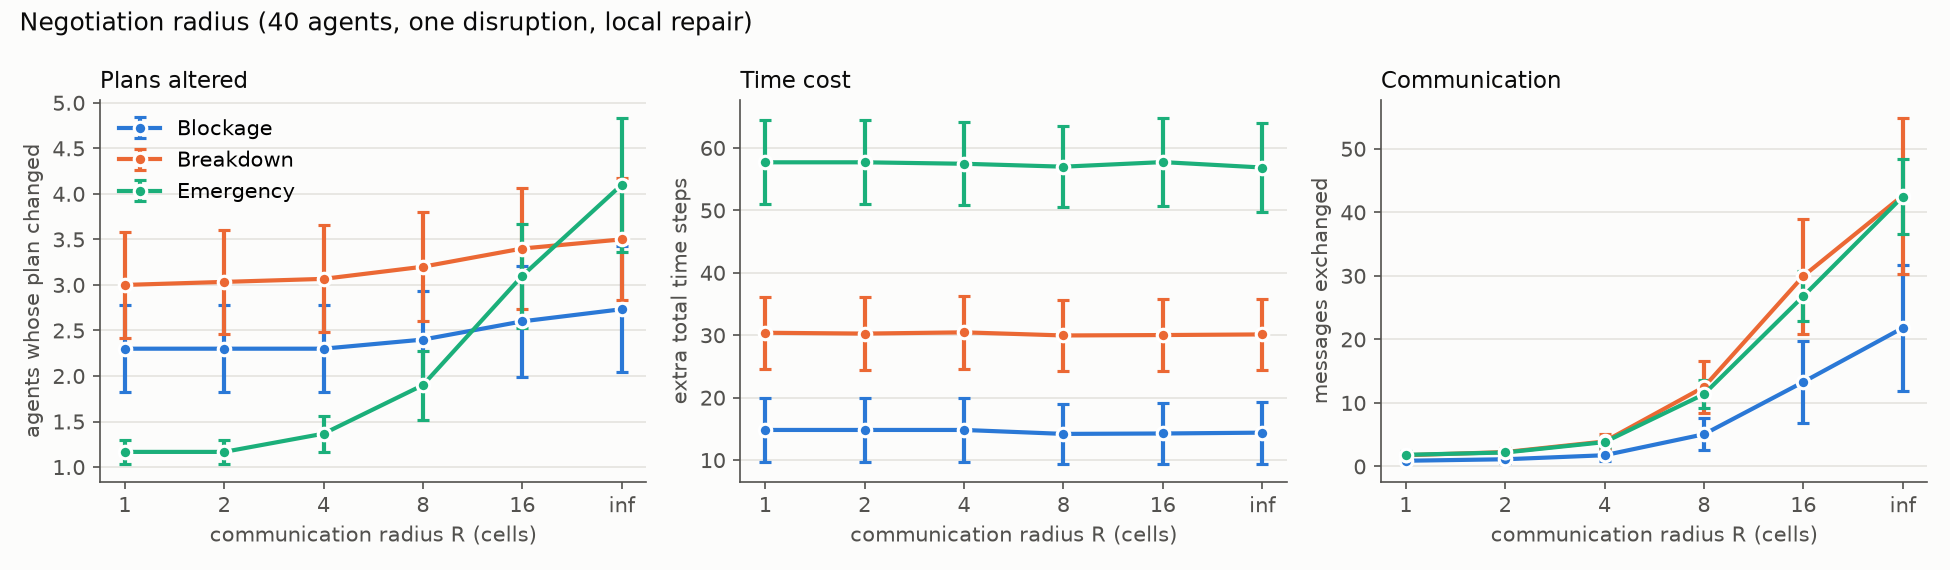
\includegraphics[width=\textwidth]{radius_ablation.png}
\caption{Effect of the communication radius $R$ (40 agents, one disruption, local repair).}
\label{fig:radius}
\end{figure}

\subsection{Simultaneous breakdowns (Exp F)}

\begin{figure}[H]
\centering
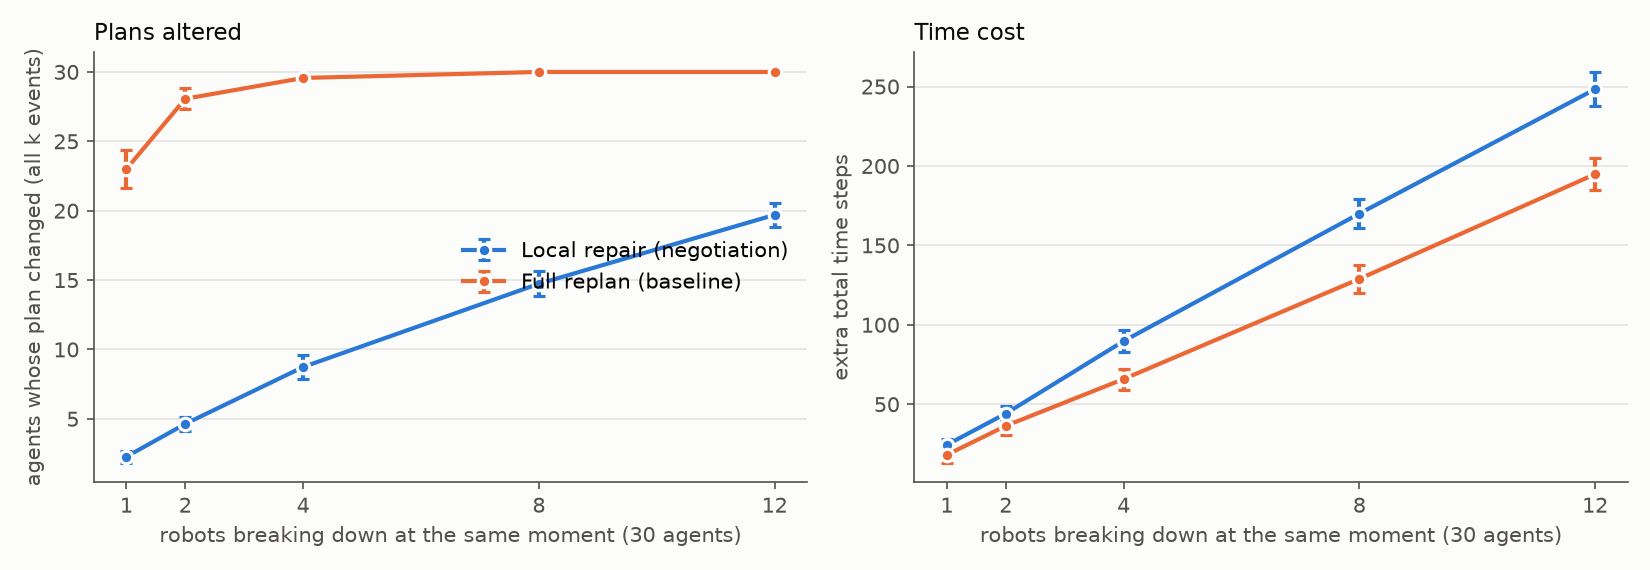
\includegraphics[width=0.9\textwidth]{simultaneous_breakdowns.png}
\caption{$k$ robots break down in the same time step (30 agents).}
\label{fig:simul}
\end{figure}

Local repair changes about 1.6--2.3 plans per broken robot (19.7 for $k=12$), while a full replan already
changes almost all 30 plans for $k=2$. The time gap grows with $k$ (248 vs.\ 195 extra steps at $k=12$),
but local repair stays about $38\times$ cheaper to compute (0.28\,s vs.\ 10.7\,s).

\subsection{Bigger warehouse and longer task lists (Exps G, H)}\label{sec:bigmap}\label{sec:tasks}

\begin{figure}[H]
\centering
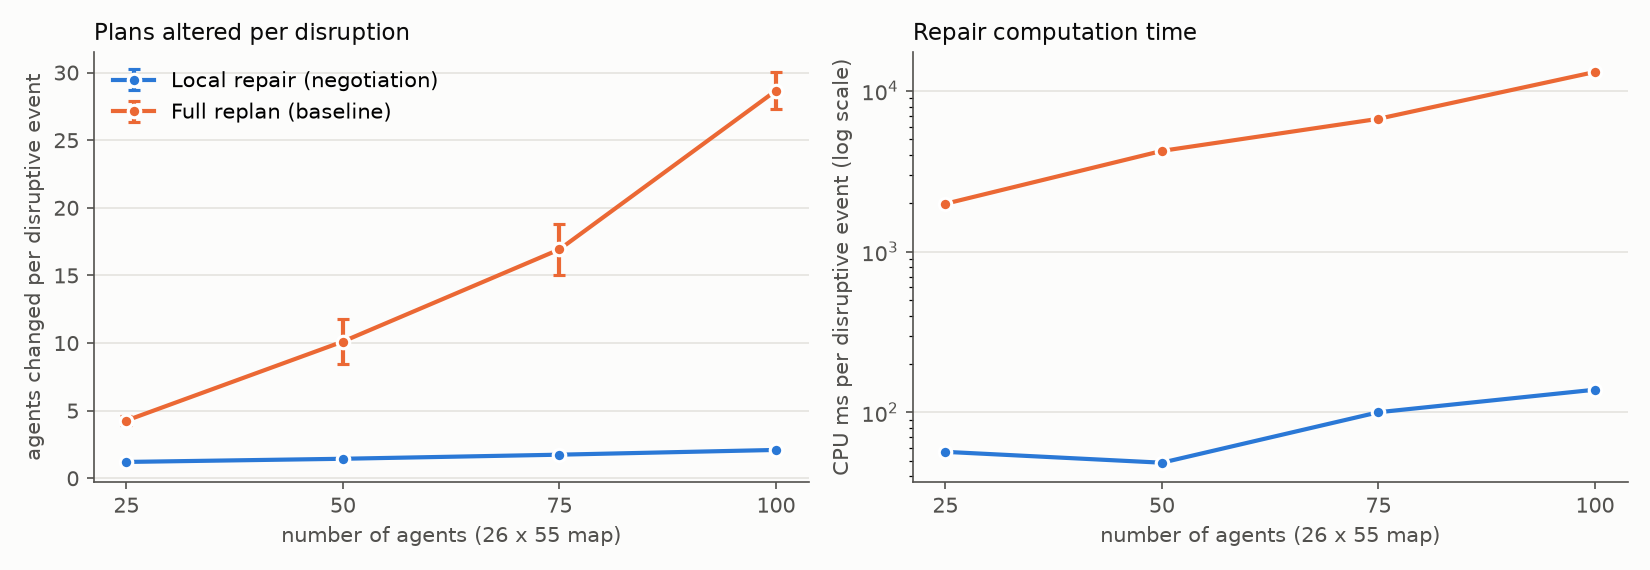
\includegraphics[width=\textwidth]{bigmap_changes.png}
\caption{Bigger $26\times55$ warehouse with up to 100 robots.}
\label{fig:bigmap}
\end{figure}

With 100 robots on the bigger map, local repair changes 2.10 plans per disruption against 28.67 for a
full replan, with only 0.4\% more total time (22{,}426 vs.\ 22{,}341). The full replan needs 13\,s per
disruption against 0.14\,s. With 1--8 tasks per robot, local repair stays at about 1.4 changed plans per
event (full replan: 4.6 to 7.8) and within 0.6\% of the full replan's total time.

% ================================================================== 6
\section{Failure Settings: Where the Agents Do Not Complete Their Tasks}\label{sec:failures}

Exp I deliberately pushes the system past its limits. A run is a \emph{success} only if every task is
delivered. A run can fail in two ways:
\begin{itemize}
  \item \textbf{Halt (deadlock):} some robots are left with no conflict-free plan. In purely local mode
  the run stops at that step and undelivered tasks count as failed.
  \item \textbf{Lost tasks:} a permanent disruption makes a task impossible (e.g.\ its pickup cell is
  blocked for good). The task is dropped and the other robots carry on.
\end{itemize}
None of the 2{,}630 runs had a collision: the system either finds a valid plan or stops; it never
executes an invalid one.

\subsection{Dense dynamic obstacles and large fleets: deadlock}

\begin{figure}[H]
\centering
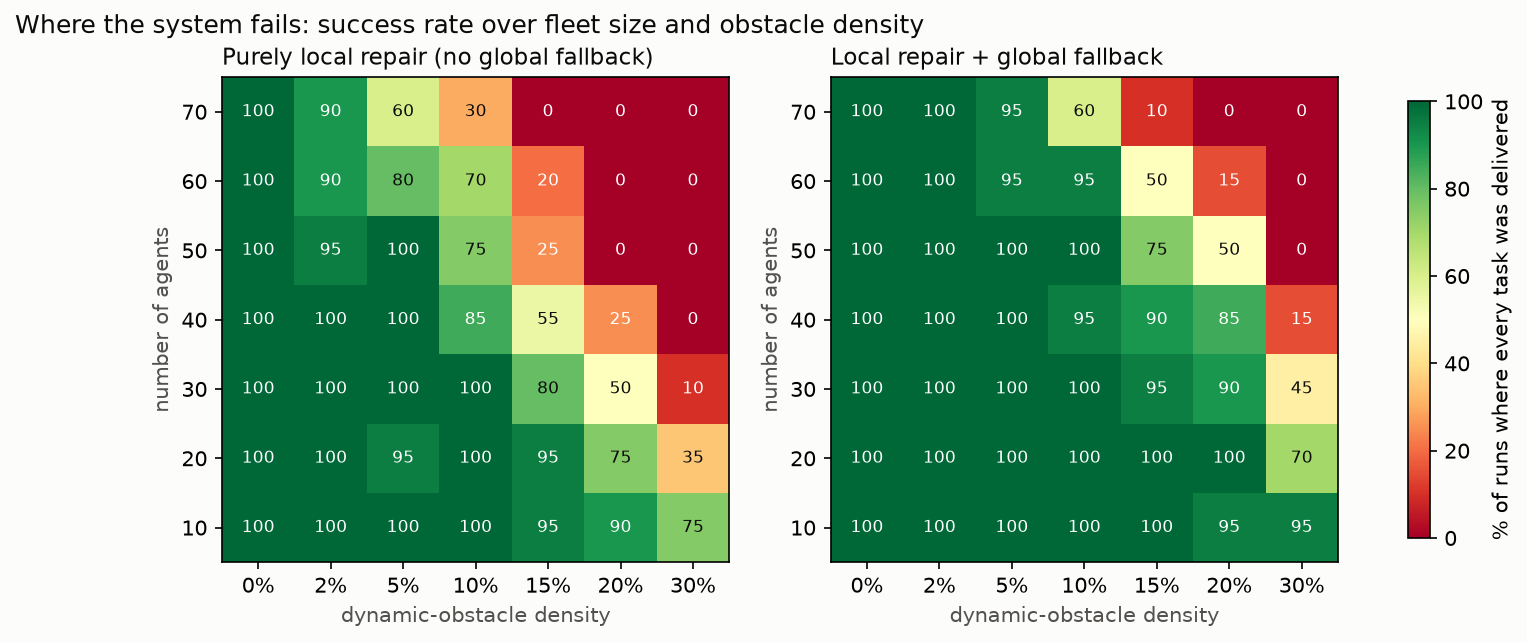
\includegraphics[width=\textwidth]{failure_heatmap.png}
\caption{Share of 20 runs in which every task was delivered, over fleet size and obstacle density. Left:
purely local repair; right: with the global fallback.}
\label{fig:heatmap}
\end{figure}

\begin{table}[H]
\centering\small
\caption{Failure settings with purely local repair.}
\label{tab:fail-density}
\begin{tabularx}{\textwidth}{@{}p{4.2cm}>{\centering\arraybackslash}X>{\centering\arraybackslash}X>{\centering\arraybackslash}X@{}}
\toprule
Fleet size & Highest $\rho$ with $\ge95\%$ success & Lowest $\rho$ where $\ge50\%$ of runs fail & Tasks delivered at $\rho=30\%$ \\
\midrule
10 robots & 15\% & $>30\%$ & 80\% \\
20 robots & 15\% & 30\% & 47\% \\
30 robots & 10\% & 20\% & 28\% \\
40 robots & 5\%  & 20\% & 7\% \\
50 robots & 5\%  & 15\% & 4\% \\
60 robots & 0\%  & 15\% & 2\% \\
70 robots (all homes used) & 0\% & 10\% & 1\% \\
\bottomrule
\end{tabularx}
\end{table}

\textbf{Why the robots fail.} At high density the blocked cells leave only one-cell-wide gaps between
shelves. Two robots meet head-on in such a gap, or a robot is boxed in between blocked cells and other
robots' committed paths. Local repair keeps all other plans fixed except the negotiating neighbours, so
when the conflict involves a chain of robots longer than the recursion depth, every local option fails. In
these deadlocks every stuck robot could still reach all its goals if it were alone on the map: the
failure is one of coordination, not reachability. Figure~\ref{fig:deadlock} shows such a deadlock.

\begin{figure}[H]
\centering
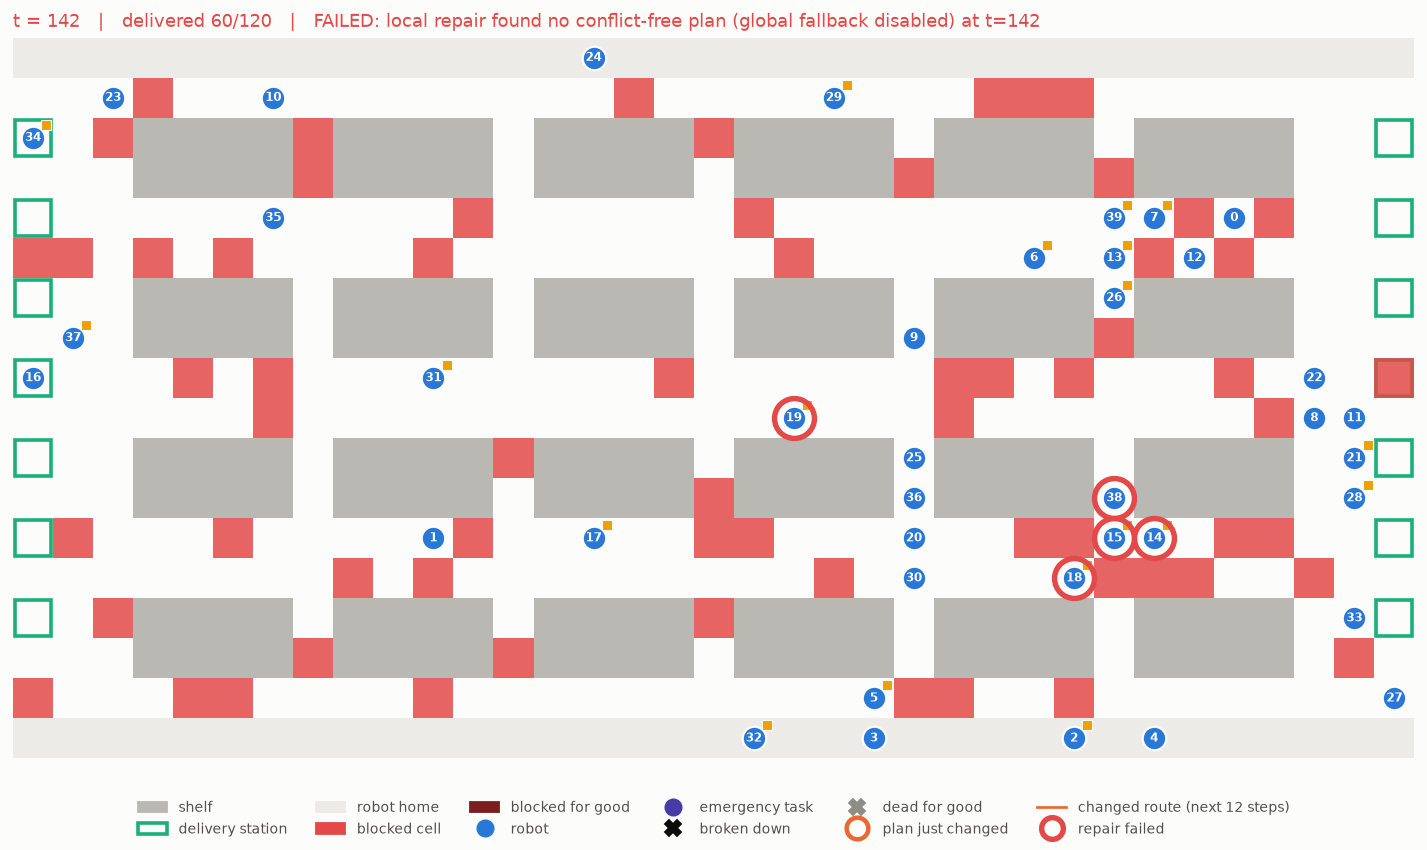
\includegraphics[width=\textwidth]{snapshot_failure_deadlock.png}
\caption{Deadlock with 40 robots at $\rho=20\%$ (purely local repair). At $t=142$ the robots ringed in
red cannot be repaired; 60 of 120 tasks were delivered.}
\label{fig:deadlock}
\end{figure}

\textbf{The global fallback widens the safe range but does not remove the failure.} It raises success
from 55\% to 90\% for 40 robots at $\rho=15\%$, and from 30\% to 60\% for 70 robots at $\rho=10\%$. At
$\rho=30\%$ with 40 or more robots, and at $\rho=20\%$ with 60 or more robots, it also fails in almost
every run, because prioritized planning is incomplete. Long blockages, by contrast, are not a failure
setting: raising the mean blockage duration from 15 to 180 steps (30 robots, $\rho=10\%$) leaves the
success rate at 95--100\%, since the robots simply detour.

\subsection{Permanent disruptions: tasks that can never be done}

\begin{figure}[H]
\centering
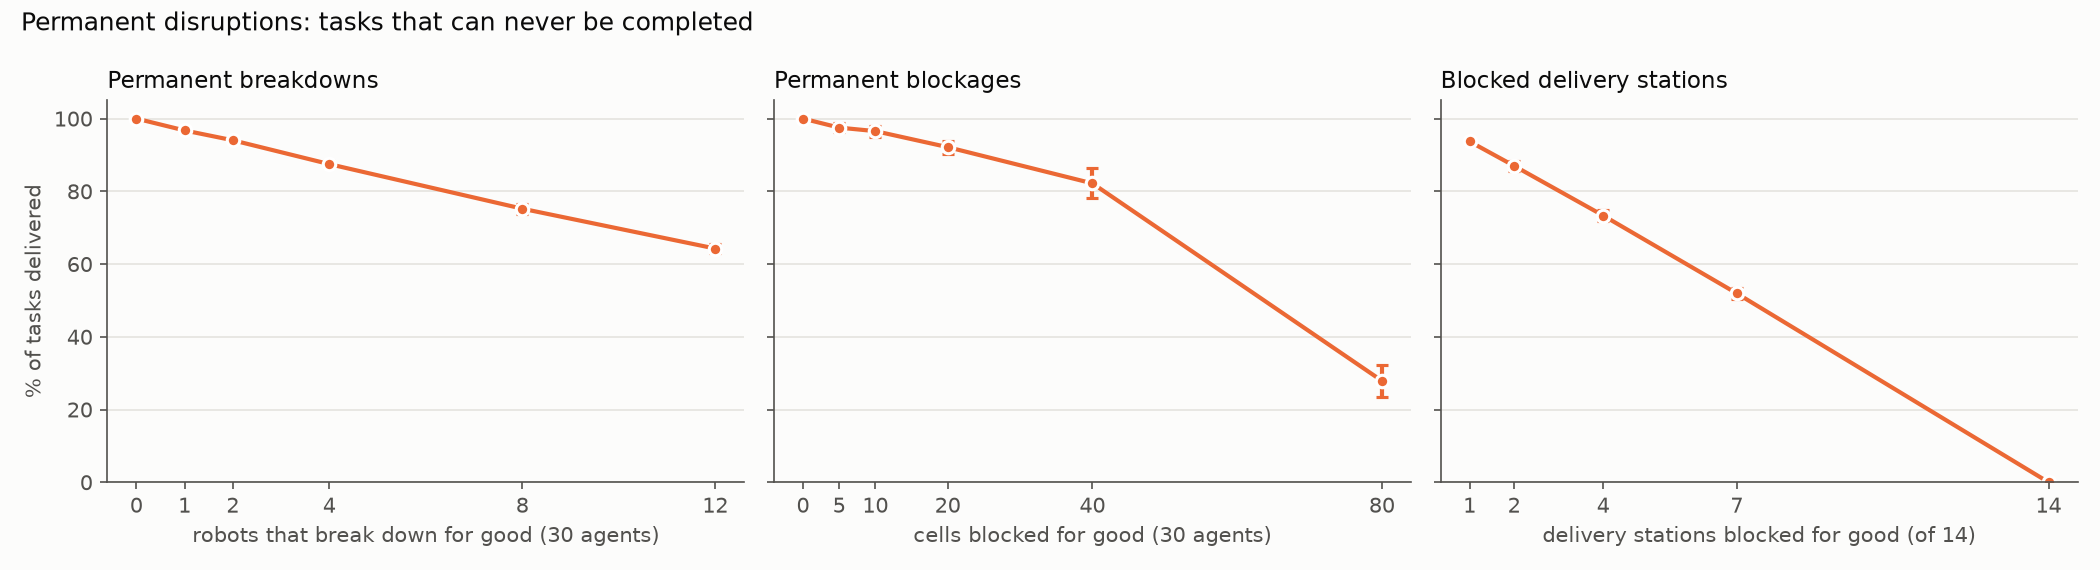
\includegraphics[width=\textwidth]{failure_permanent.png}
\caption{Share of tasks delivered under permanent breakdowns, permanent blockages and blocked delivery
stations (30 robots, 90 tasks, 30 seeds).}
\label{fig:permanent}
\end{figure}

\begin{table}[H]
\centering\small
\caption{Permanent disruptions (30 robots, 90 tasks).}
\label{tab:fail-perm}
\begin{tabularx}{\textwidth}{@{}p{5.2cm}p{2.6cm}Y@{}}
\toprule
Setting & Tasks delivered & Main cause of lost tasks \\
\midrule
1 robot breaks down for good & 96.7\% & The dead robot's own tasks; tasks whose cell it occupies \\
4 robots break down for good & 87.5\% & Same (11.3 tasks lost) \\
12 robots break down for good & 64.3\% & Same (32 tasks lost) \\
5 cells blocked for good & 97.5\% & Blocked cell is a pickup cell or station \\
40 cells blocked for good & 82.2\% & Same, plus a few cells walled off \\
80 cells blocked for good (22\%) & 27.9\% & 93\% of runs deadlock in single-lane passages \\
1 of 14 stations blocked & 93.7\% & Every task assigned to that station \\
7 of 14 stations blocked & 51.9\% & Same \\
14 of 14 stations blocked & 0\% & No delivery is possible \\
\bottomrule
\end{tabularx}
\end{table}

The system has no task reallocation, so a dead robot's undelivered tasks (about 2.7--2.9 per robot) are
lost, and each task has one fixed pickup cell and one fixed station. Figure~\ref{fig:perm-snap} shows the
end of such a run.

\begin{figure}[H]
\centering
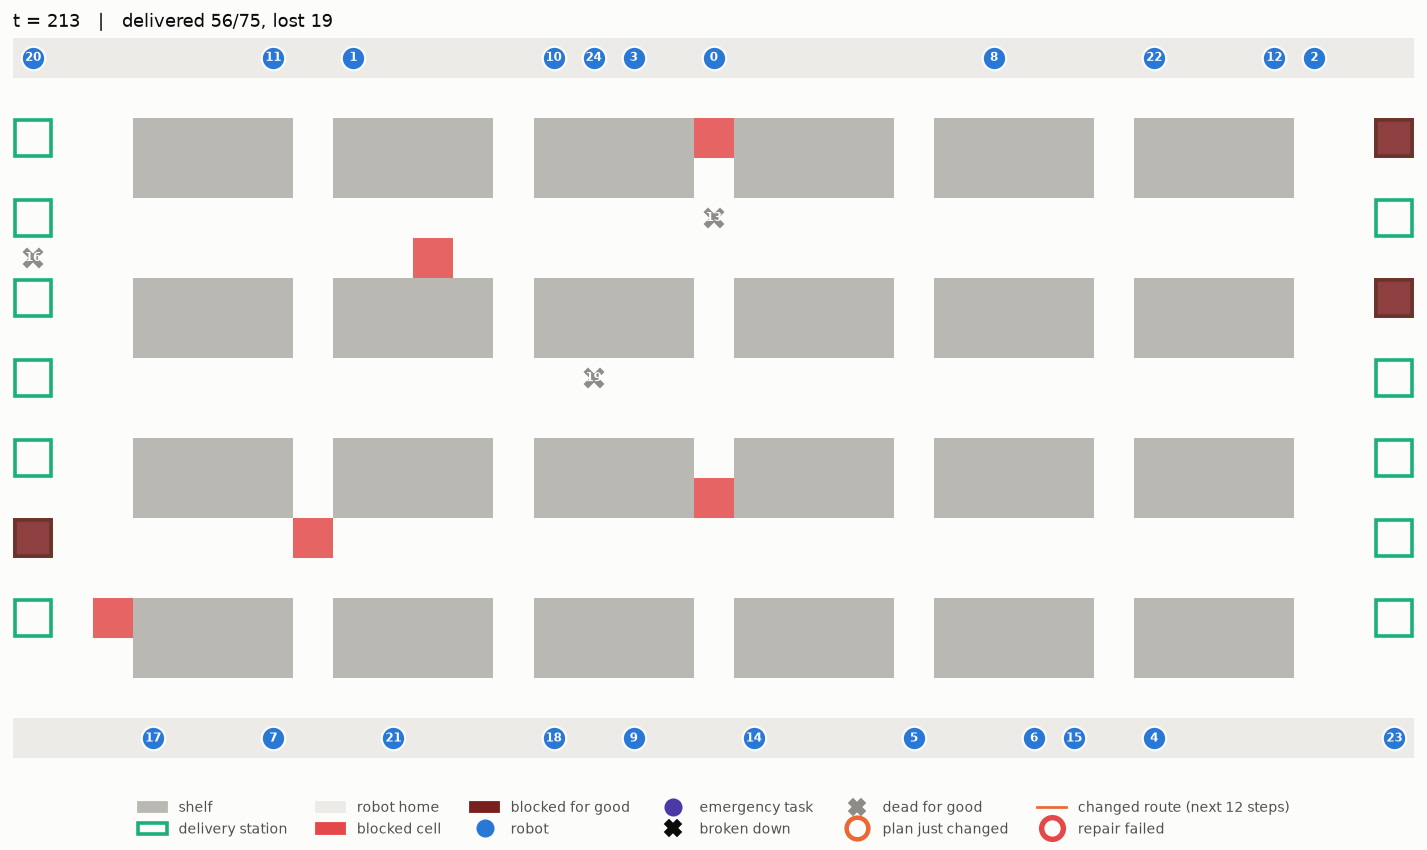
\includegraphics[width=\textwidth]{snapshot_failure_permanent.png}
\caption{25 robots, 3 robots dead for good (grey crosses) and 3 stations blocked for good (dark red): 56
of 75 tasks are delivered.}
\label{fig:perm-snap}
\end{figure}

\subsection{Summary of failure settings}

\begin{table}[H]
\centering\small
\caption{Settings in which the agents do not complete their tasks.}
\label{tab:fail-summary}
\begin{tabularx}{\textwidth}{@{}p{0.4cm}p{7.2cm}Y@{}}
\toprule
\# & Setting & What happens \\
\midrule
1 & Purely local repair with $\rho\ge20\%$ and $\ge30$ robots, $\rho\ge15\%$ and $\ge50$ robots, or
$\rho\ge10\%$ and 70 robots & Half or more of the runs deadlock and halt \\
2 & $\rho=30\%$ with $\ge40$ robots, or $\rho=20\%$ with $\ge60$ robots, even with the global fallback &
85--100\% of runs deadlock; global replanning fails too \\
3 & Fleet that fills every home cell (70 robots) & Fails from $\rho=2$--$5\%$ \\
4 & A robot breaks down for good & Its remaining tasks are lost; no reallocation \\
5 & A pickup cell or station blocked for good & Every task using it is lost \\
6 & $\ge20\%$ of free cells blocked for good & Remaining passages become single lanes; runs deadlock \\
\bottomrule
\end{tabularx}
\end{table}

Possible remedies (not implemented): task reallocation by auction when a robot dies and re-routing to the
nearest open station (failures 4--5); a complete MAPF method such as Conflict-Based Search, or
push-and-swap style backing out of single lanes, as the last local resort (failures 1--3, 6); and
admission control that limits active robots in congested regions.

% ================================================================== 7
\section{Graphical Demonstration}\label{sec:vis}

\texttt{visualize.py} renders animated GIFs of the simulation (Table~\ref{tab:gifs}). In the animations a
red cell is a blockage, dark red is blocked for good, a black cross is a broken robot, a grey cross a
robot dead for good, violet a robot on an emergency task, an orange ring and line mark a robot whose plan
just changed (with its next 12 steps), and a thick red ring marks a robot whose repair failed.
Figure~\ref{fig:snapshots} shows one repair of each disruption type.

\begin{table}[H]
\centering\small
\caption{Animations in \texttt{results/gifs/}.}
\label{tab:gifs}
\begin{tabularx}{\textwidth}{@{}p{4.2cm}Y@{}}
\toprule
File & Scenario \\
\midrule
\texttt{demo.gif} & 15 robots, $\rho=2\%$, 3 breakdowns, 2 emergencies \\
\texttt{blockages.gif} & 20 robots, blockages only, $\rho=5\%$ \\
\texttt{breakdowns.gif} & 25 robots, 6 breakdowns \\
\texttt{emergencies.gif} & 20 robots, 4 emergency tasks \\
\texttt{dense.gif} & 50 robots, $\rho=2\%$ \\
\texttt{bigmap.gif} & 60 robots on the $26\times55$ map \\
\texttt{compare.gif} & Same 25-robot scenario: local repair (top) vs.\ full replan (bottom) \\
\texttt{failure\_deadlock.gif} & \textbf{Failure:} 40 robots, $\rho=20\%$, deadlock at $t=142$ \\
\texttt{failure\_permanent.gif} & \textbf{Failure:} 3 robots dead and 3 stations blocked for good \\
\bottomrule
\end{tabularx}
\end{table}

\begin{figure}[H]
\centering
\begin{subfigure}{\textwidth}\centering
  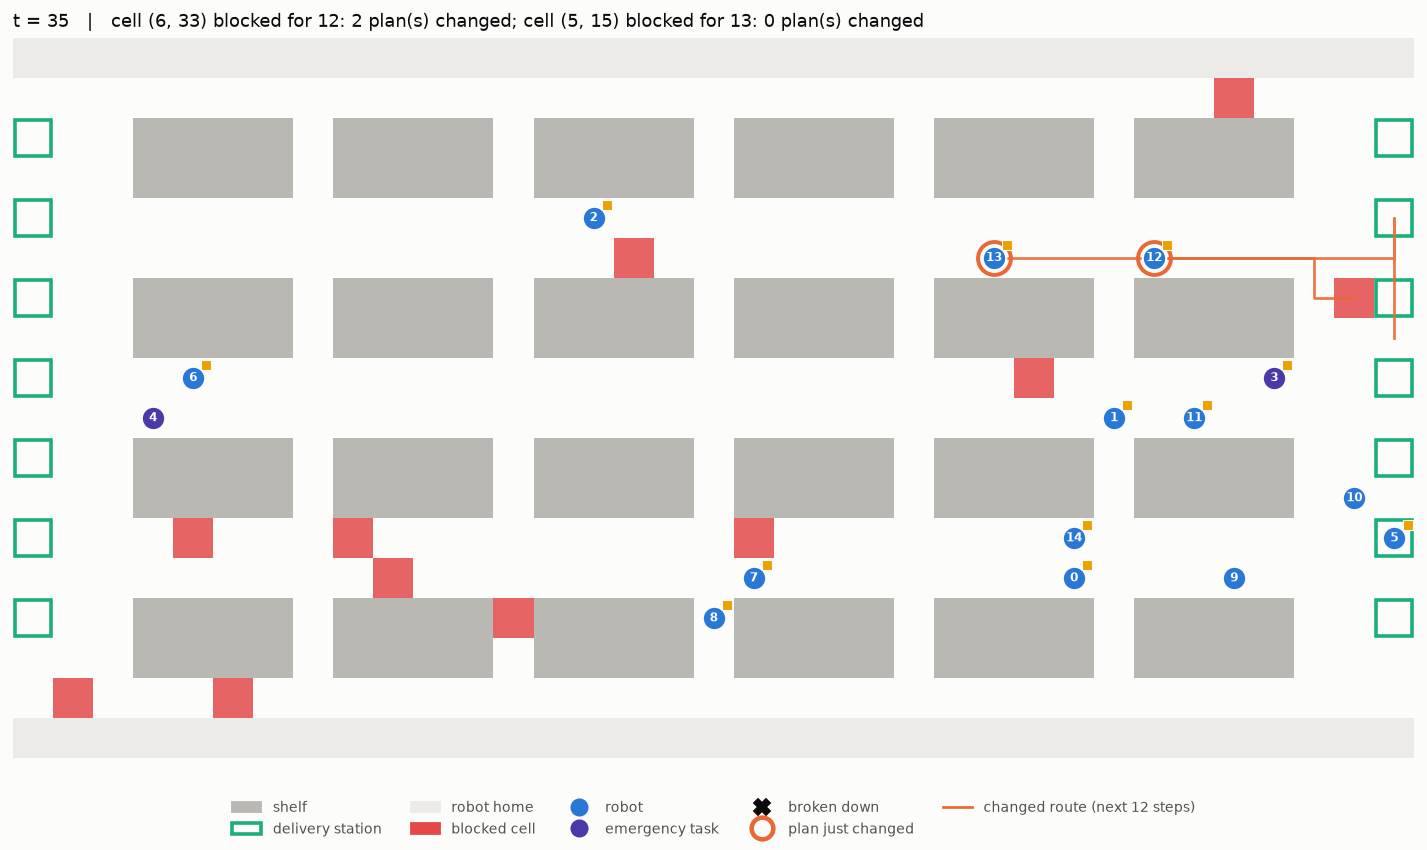
\includegraphics[width=0.7\textwidth]{snapshot_blocked.png}
  \caption{Cell blockage: the blocked robot detours.}
\end{subfigure}\\[4pt]
\begin{subfigure}{\textwidth}\centering
  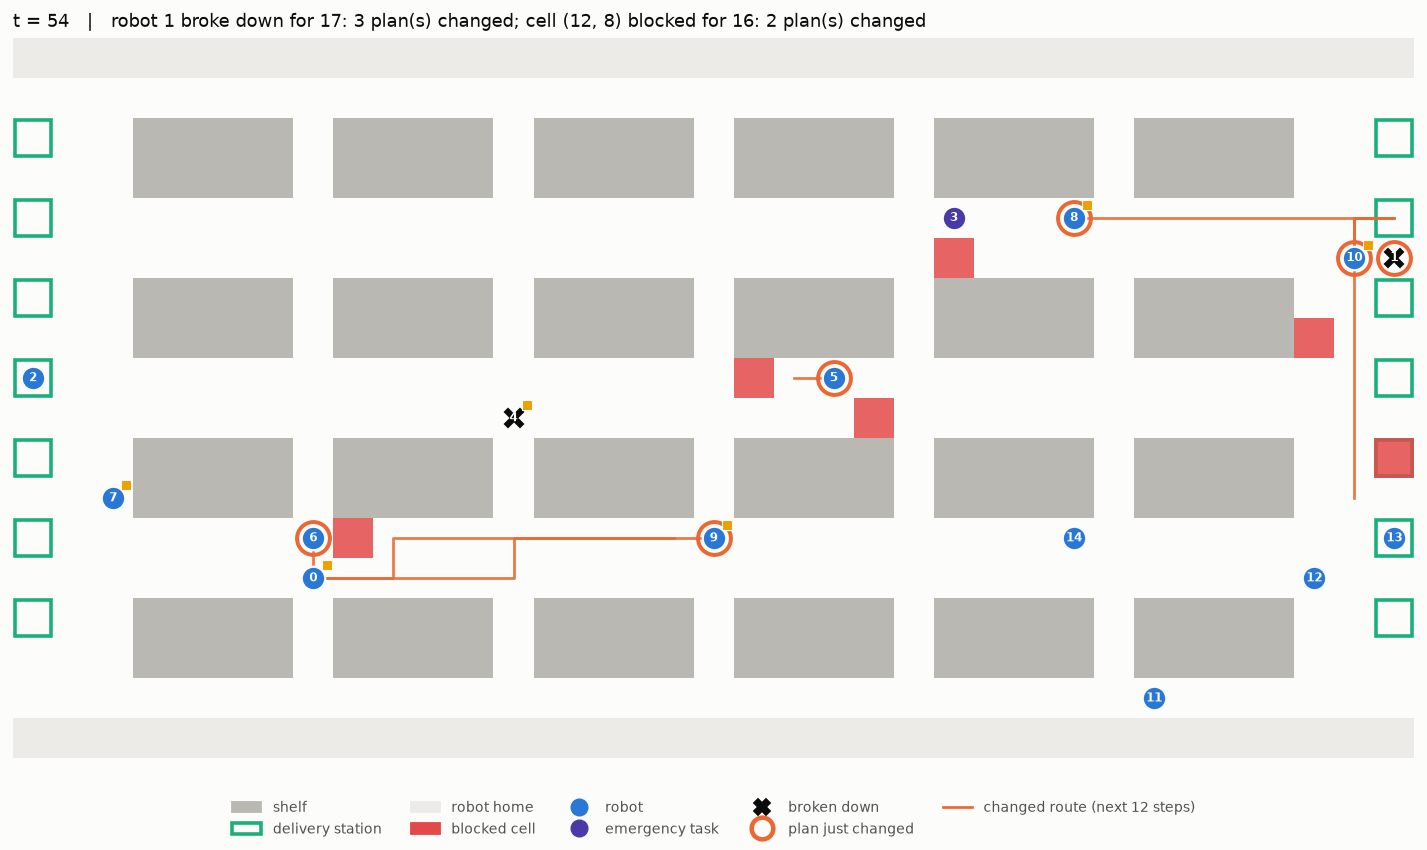
\includegraphics[width=0.7\textwidth]{snapshot_broke.png}
  \caption{Breakdown: robots whose routes cross the broken robot repair around it.}
\end{subfigure}\\[4pt]
\begin{subfigure}{\textwidth}\centering
  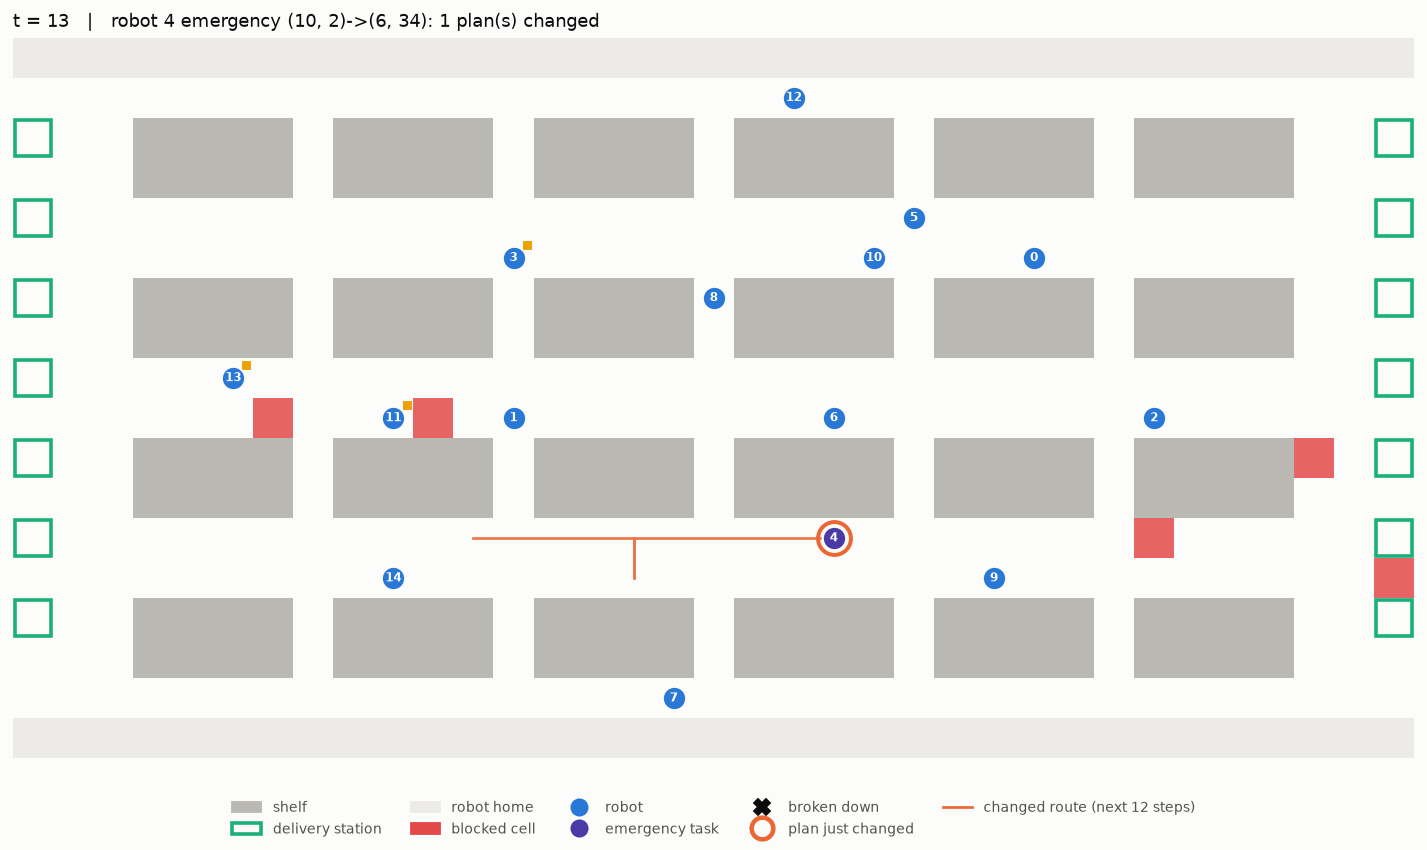
\includegraphics[width=0.7\textwidth]{snapshot_emergency.png}
  \caption{Emergency task: the emergency robot gets a fast route; neighbours give way if needed.}
\end{subfigure}
\caption{Snapshots of local repairs from \texttt{demo.gif}.}
\label{fig:snapshots}
\end{figure}

% ================================================================== 8
\section{Discussion and Limitations}

\begin{itemize}
  \item \textbf{Plan modification is local.} For one disruption, 1--3.5 plans change as the fleet grows
  to 50 robots and about 2 with 100 robots, nearly flat across densities and task-list lengths. A full
  replan changes most plans, and its cost grows with $N$.
  \item \textbf{Trade-off.} Local repair gives up a little total time (at most 1.1\% over whole runs) for
  stable plans and cheap computation. Stable plans matter in practice, because every plan change must be
  sent to a robot and may invalidate bookings of lifts, doors or chargers.
  \item \textbf{Tuning.} Negotiating more (smaller $\tau$, larger $R$) changes more plans without saving
  time; the remaining gap comes from keeping the unaffected robots' priorities fixed.
  \item \textbf{Completeness.} Prioritized planning and repairs that keep other plans fixed are not
  complete. Section~\ref{sec:failures} shows where this matters: high density with large fleets, and
  permanent disruptions.
  \item \textbf{Assumptions.} Blockage durations are known when they appear; communication within the
  radius is reliable and instantaneous; a robot carries one object at a time.
\end{itemize}

% ================================================================== 9
\section{Conclusion}

We built a warehouse simulator in which robots plan with prioritized Space-Time A* and respond to
blockages, breakdowns and emergency tasks through local, negotiation-based plan repair, without
re-invoking the multi-agent planner. Across 3{,}320 runs, a single disruption changes the plans of only
1.1--3.5 robots (against up to 45 for a full replan), the total time stays within 1.1\% of a full replan,
and repair is one to two orders of magnitude cheaper to compute. The method fails when dynamic obstacles
are dense and the fleet is large, where robots deadlock in single-lane gaps, and under permanent
disruptions, where some tasks become impossible. Task reallocation and a complete last-resort solver are
the natural next steps.

% ================================================================== refs
% \begin{thebibliography}{9}
% \bibitem{silver2005} D.~Silver. Cooperative pathfinding. In \emph{Proc.\ AIIDE}, 2005.
% \bibitem{stern2019} R.~Stern et al. Multi-agent pathfinding: definitions, variants, and benchmarks. In
% \emph{Proc.\ SoCS}, 2019.
% \bibitem{sharon2015} G.~Sharon, R.~Stern, A.~Felner, N.~Sturtevant. Conflict-based search for optimal
% multi-agent pathfinding. \emph{Artificial Intelligence}, 219:40--66, 2015.
% \bibitem{luna2011} R.~Luna, K.~Bekris. Push and swap: fast cooperative path-finding with completeness
% guarantees. In \emph{Proc.\ IJCAI}, 2011.
% \bibitem{ma2017} H.~Ma, J.~Li, T.~K.~S.~Kumar, S.~Koenig. Lifelong multi-agent path finding for online
% pickup and delivery tasks. In \emph{Proc.\ AAMAS}, 2017.
% \end{thebibliography}

% ================================================================== appendix
\appendix
\section{Code Structure and Reproduction}

\begin{table}[H]
\centering\small
\begin{tabularx}{\textwidth}{@{}p{6cm}Y@{}}
\toprule
File & Contents \\
\midrule
\texttt{warehouse/grid.py} & Grid map, dynamic and permanent blockages, BFS heuristic \\
\texttt{warehouse/reservation.py} & Space-time reservation table \\
\texttt{warehouse/planner.py} & Space-Time A*, multi-leg routes, prioritized planning \\
\texttt{warehouse/repair.py} & Local repair L0/L1/L2 with negotiation and rollback \\
\texttt{warehouse/baseline.py} & Full prioritized replan (baseline) \\
\texttt{warehouse/simulator.py} & Execution, disruption injection, failure detection, collision checks \\
\texttt{experiments/run\_experiments.py} & Experiments A--I, CSVs and figures \\
\texttt{visualize.py} & GIF animations and snapshots \\
% \texttt{tests/} & 12 unit and end-to-end tests \\
\bottomrule
\end{tabularx}
\end{table}

\begin{verbatim}
python3 -m venv .venv && .venv/bin/pip install -r requirements.txt
.venv/bin/pytest -q                              # 12 tests
.venv/bin/python experiments/run_experiments.py  # experiments A-I
.venv/bin/python visualize.py --preset all       # the nine GIFs
\end{verbatim}

\end{document}
